\documentclass[a4paper]{scrbook} 
\usepackage{pgfplots}
\pgfplotsset{compat=1.16}% <- aktuelle Version ist 1.16

\pgfplotsset{ 
   cycle list/.define={my marks}{ 
      every mark/.append style={solid,fill=\pgfkeysvalueof{/pgfplots/mark list fill}},mark=*\\ 
      every mark/.append style={solid,fill=\pgfkeysvalueof{/pgfplots/mark list fill}},mark=star\\ 
      every mark/.append style={solid,fill=\pgfkeysvalueof{/pgfplots/mark list fill}},mark=square\\ 
      every mark/.append style={solid,fill=\pgfkeysvalueof{/pgfplots/mark list fill}},mark=+\\   
      every mark/.append style={solid,fill=\pgfkeysvalueof{/pgfplots/mark list fill}},mark=triangle\\ 
      every mark/.append style={solid,fill=\pgfkeysvalueof{/pgfplots/mark list fill}},mark=x\\   
      every mark/.append style={solid,fill=\pgfkeysvalueof{/pgfplots/mark list fill}},mark=pentagon\\ 
      every mark/.append style={solid,fill=\pgfkeysvalueof{/pgfplots/mark list fill}},mark=o\\ 
      every mark/.append style={solid,fill=\pgfkeysvalueof{/pgfplots/mark list fill}},mark=diamond\\ 
   }, 
  cycle list/.define={my colors}{red,gray,blue,green!70!black},
  cycle multiindex* list={
    my marks\nextlist 
    my colors\nextlist
  }
}

\begin{document} 
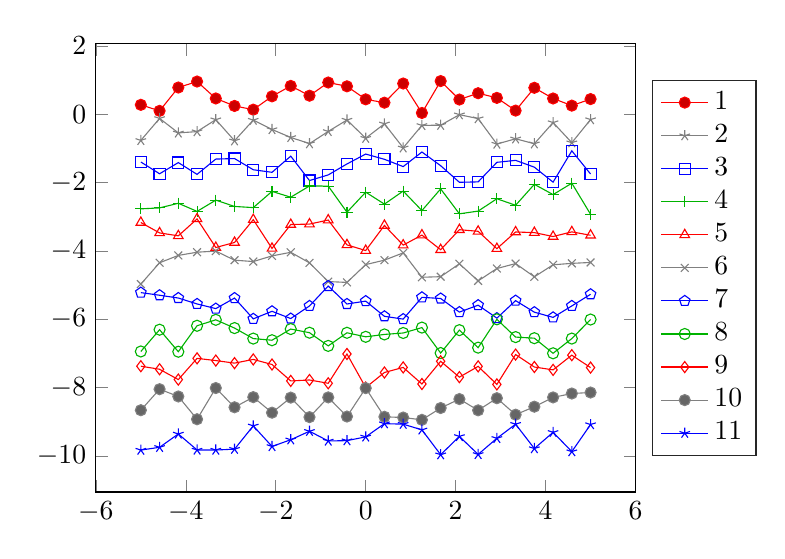
\begin{tikzpicture} 
  \begin{axis}[ 
    legend style={at={(1.03,0.5)}, anchor=west, legend cell align=left, align=left, draw=white!15!black} 
  ] 
  \addplot {rnd};\addlegendentry{1}
  \addplot {rnd-1};\addlegendentry{2}
  \addplot {rnd-2};\addlegendentry{3}
  \addplot {rnd-3};\addlegendentry{4}
  \addplot {rnd-4};\addlegendentry{5}
  \addplot {rnd-5};\addlegendentry{6}
  \addplot {rnd-6};\addlegendentry{7}
  \addplot {rnd-7};\addlegendentry{8}
  \addplot {rnd-8};\addlegendentry{9}
  \addplot {rnd-9};\addlegendentry{10}
  \addplot {rnd-10};\addlegendentry{11}
  \end{axis} 
\end{tikzpicture} 
\end{document}